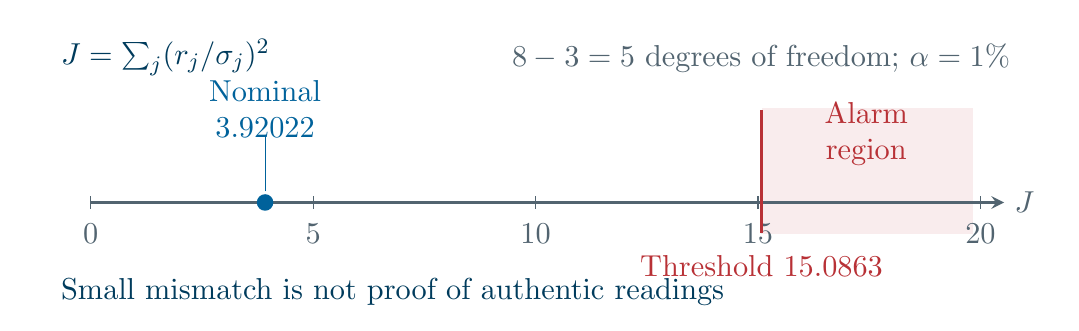
\begin{tikzpicture}[x=1cm,y=1cm,font=\fontsize{11}{13}\selectfont,>=stealth]
\definecolor{IEEEBlue}{HTML}{00629B}
\definecolor{Cyan}{HTML}{00A6B2}
\definecolor{Navy}{HTML}{003B5C}
\definecolor{Slate}{HTML}{526470}
\definecolor{CaseRed}{HTML}{B83136}
\path[use as bounding box] (0,0) rectangle (13,3.5);
\node[anchor=west,text=Navy] at (.3,3.12) {$J=\sum_j(r_j/\sigma_j)^2$};
\node[anchor=east,text=Slate] at (12.6,3.12) {$8-3=5$ degrees of freedom; $\alpha=1\%$};
\fill[CaseRed!9] (9.32,.88) rectangle (12,2.48);
\draw[->,Slate,line width=1pt] (.8,1.28)--(12.4,1.28) node[right] {$J$};
\foreach \x/\v in {.8/0,3.625/5,6.45/10,9.275/15,12.1/20} {\draw[Slate] (\x,1.2)--(\x,1.36);\node[below,text=Slate] at (\x,1.13) {\v};}
\draw[CaseRed,line width=1.3pt] (9.32,.89)--(9.32,2.46);
\fill[IEEEBlue] (3.015,1.28) circle (.105);
\draw[IEEEBlue] (3.015,1.42)--(3.015,2.12);
\node[text=IEEEBlue,align=center] at (3.015,2.47) {Nominal\\$3.92022$};
\node[text=CaseRed,align=center] at (10.65,2.15) {Alarm\\region};
\node[text=CaseRed] at (9.32,.47) {Threshold $15.0863$};
\node[anchor=west,text=Navy] at (.3,.15) {Small mismatch is not proof of authentic readings};
\end{tikzpicture}%
